\section{Skin}
The skin is a complex organ a ~\cite{elin2018}, it is interactive, self renewing and represents the first and primary defense line against hostile environment, and it has several characteristics such as selective absorption, auto regeneration when injured, barrier to water loss, touch sensitivity ...etc. ~\cite{joseph2020}. It represents the largest sensory organ (15\% of total body weight and a total area of 1.86 m²) ~\cite{sarah2021}, it has a highly adaptive structure that makes it vital for the survival of the human body, the balance between its static and dynamic properties makes it highly adaptive to the variations of the outer world ~\cite{eliana2022}.

\subsection{Skin Anatomy}
The skin is primary composed of 3 main layers as shown in the figure ~\ref{fig:skin}, each layer has its unique properties and functions ~\cite{sarah2021}.
\begin{description}
\item[Epidermis] The outermost layer which is constantly regenerating, and it contains the pigment melanin that determines the skin color, and it also represents a physical and biological barrier.
\item[Dermis] The middle layer, it supports the flexibility and gives strength to the epidermis, and it is mainly composed of connective tissue.
\item[Hypodermis] The last layer which is composed of subcutaneous fat which gives it its properties of being a main support of the overall structure of the skin and shock absorption.
\end{description}

%-----------figure skin structure/anatomy ----------------
\begin{figure}[htbp]
\begin{center}
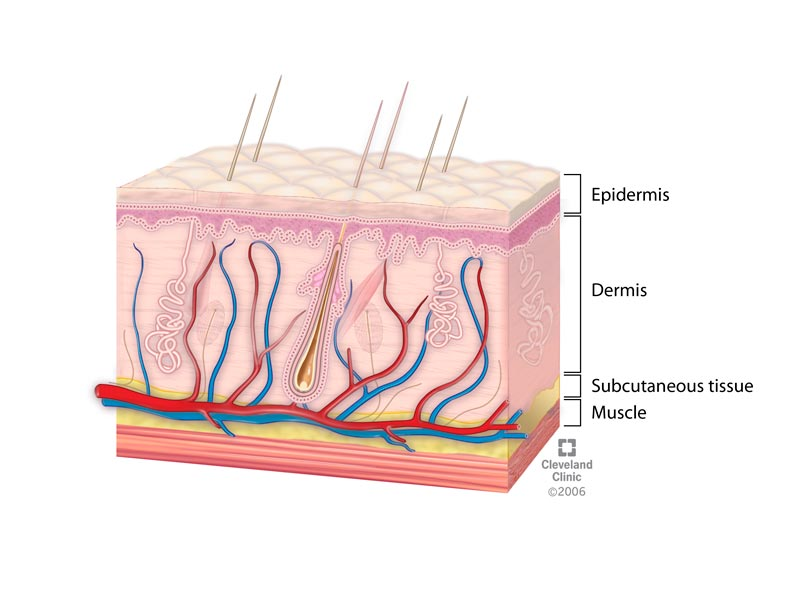
\includegraphics[width=15cm]{./chapter-01-general-medical-information/skin-anatomy.jpg}
\end{center}
\caption{Skin Anatomy ~\cite{fig-skin}}
\label{fig:skin}
\end{figure}

\subsection{Other entities also contained in the skin}
\begin{description}
\item[Hair]  provides protection against minor trauma, thermoregulation and filtering functions such as nasal hair and eyelashes
\item[Sweat Glands] it is found across the entire body, it provides lubrication, temperature regulation and salt and water balance.
\end{description}
their anatomies are shown in the figure ~\ref{fig:hair}

%-------------figure hair sweat glands-----------------------------
\begin{figure}[htbp]
\begin{center}
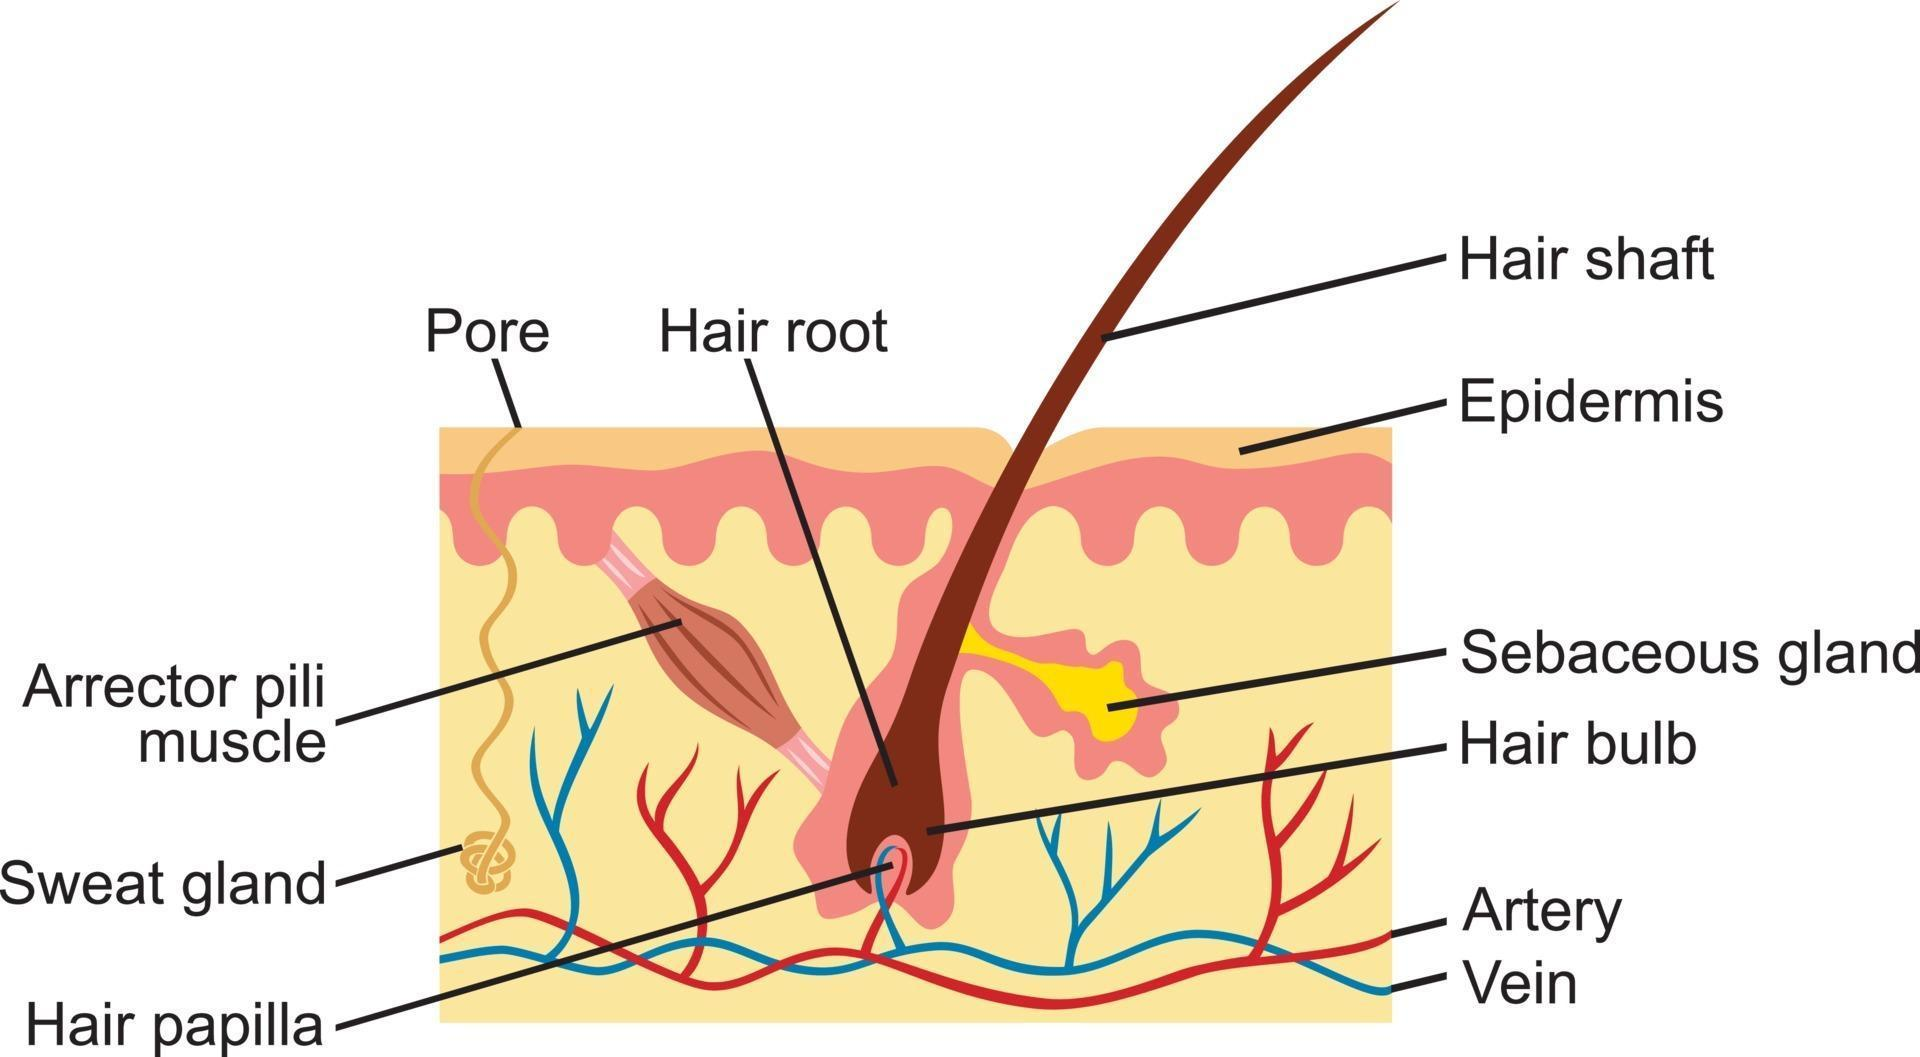
\includegraphics[width=15cm]{./chapter-01-general-medical-information/hair-sweat-gland.jpg}
\end{center}
\caption{Hair and Sweat Glands Anatomy ~\cite{fig-hair}}
\label{fig:hair}
\end{figure}


\subsection{Functions of the Skin}
The skin has 6 main functions that can be summarized as follows~\cite{sarah2021}
\begin{description}
\item[Protection] \hfill \\
            The skin is a direct interface between the internal organs and the environment, so it works as a protective barrier against harmful objects and pathogens (innate/adaptive immunity and ultraviolet light protection  ~\cite{joseph2020}) as shown in figure ~\ref{fig:barrier}.
            
\item[Thermostat] \hfill \\
            The skin works as a thermoregulator to keep the body at the optimal temperature of 37 C°, to achieve that is uses multiple strategies such as insensible perspiration, sweating ...etc.
\item[Neural relay network] \hfill \\
            The skin contains a dense network of neural endings that works as receptors to various signals and provides sensations for touch, temperature and pain.
\item[Expression and communication] \hfill \\
            A more social function
            is the ability for skin to enable individuals to display
            emotions. It acts as an indicator of one’s physical state.
            Skin is an important component of the stress response as it
            acts as an immediate stress perceiver and as a target of
            stress responses.
            The skin also works as a social tool for interactions between human beings by indicating the physical state of the individual and by showing sign of stress.
\item[Water storage] \hfill \\
            This skin works as a conservative barrier against water and body fluids' leakage (18-20\% of total body water) as shown in figure ~\ref{fig:barrier}.
\item[Synthesis of vitamin D] \hfill \\
            The skin represents the main site of vitamin D production when exposed to the sun, it exists in the plasma membranes of basal and suprabasal keratinocytes in its inactive form then it is converted to previtamin D3 then to vitamin D in the liver and kidneys  ~\cite{joseph2020} as shown in figure ~\ref{fig:vitaminD}.
\end{description}
        %----------figure skin protective barrier-------------
\begin{figure}[htbp]
\begin{center}
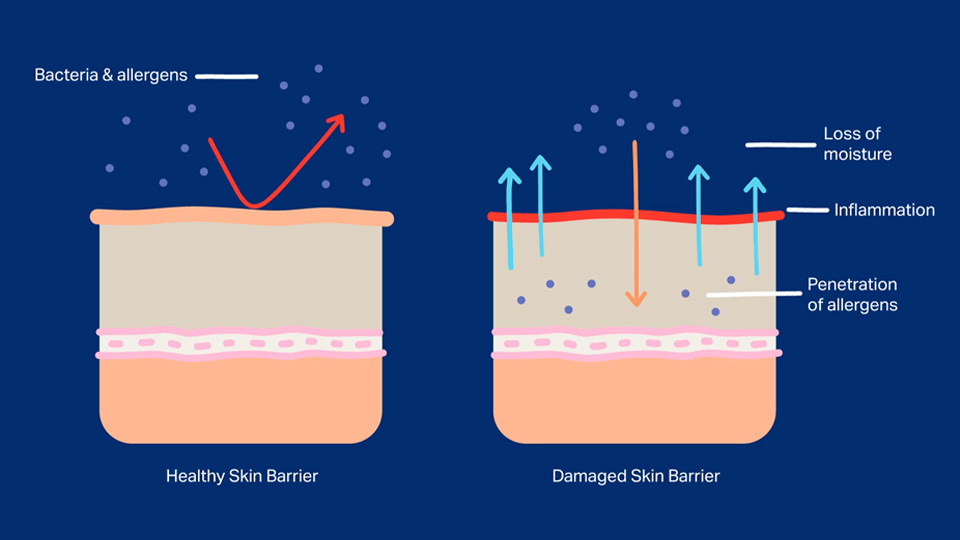
\includegraphics[width=15cm]{./chapter-01-general-medical-information/protective-barrier.jpg}
\end{center}
\caption{Protective/moisture Barrier Functions ~\cite{protectiveBarrier}}
\label{fig:barrier}
\end{figure}
        %-----------figure skin vitamin D-----------------
\begin{figure}[htbp]
\begin{center}
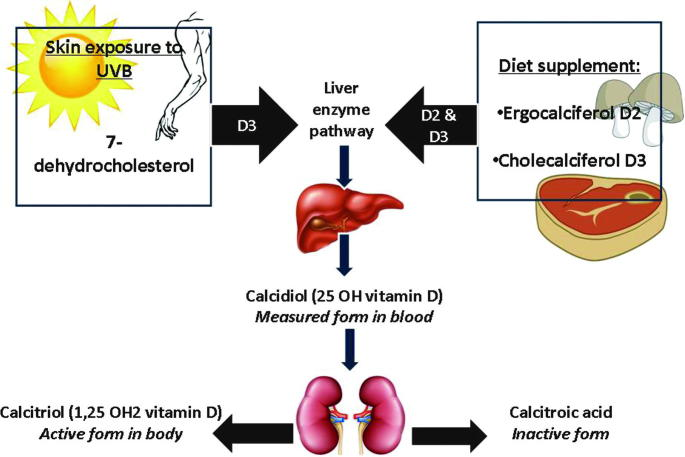
\includegraphics[width=10cm]{./chapter-01-general-medical-information/vitaminD.jpg}
\end{center}
\caption{Hair and Sweat Glands Anatomy ~\cite{vitaminD}}
\label{fig:vitaminD}
\end{figure}

